\documentclass[1p]{elsarticle_modified}
%\bibliographystyle{elsarticle-num}

%\usepackage[colorlinks]{hyperref}
%\usepackage{abbrmath_seonhwa} %\Abb, \Ascr, \Acal ,\Abf, \Afrak
\usepackage{amsfonts}
\usepackage{amssymb}
\usepackage{amsmath}
\usepackage{amsthm}
\usepackage{scalefnt}
\usepackage{amsbsy}
\usepackage{kotex}
\usepackage{caption}
\usepackage{subfig}
\usepackage{color}
\usepackage{graphicx}
\usepackage{xcolor} %% white, black, red, green, blue, cyan, magenta, yellow
\usepackage{float}
\usepackage{setspace}
\usepackage{hyperref}

\usepackage{tikz}
\usetikzlibrary{arrows}

\usepackage{multirow}
\usepackage{array} % fixed length table
\usepackage{hhline}

%%%%%%%%%%%%%%%%%%%%%
\makeatletter
\renewcommand*\env@matrix[1][\arraystretch]{%
	\edef\arraystretch{#1}%
	\hskip -\arraycolsep
	\let\@ifnextchar\new@ifnextchar
	\array{*\c@MaxMatrixCols c}}
\makeatother %https://tex.stackexchange.com/questions/14071/how-can-i-increase-the-line-spacing-in-a-matrix
%%%%%%%%%%%%%%%

\usepackage[normalem]{ulem}

\newcommand{\msout}[1]{\ifmmode\text{\sout{\ensuremath{#1}}}\else\sout{#1}\fi}
%SOURCE: \msout is \stkout macro in https://tex.stackexchange.com/questions/20609/strikeout-in-math-mode

\newcommand{\cancel}[1]{
	\ifmmode
	{\color{red}\msout{#1}}
	\else
	{\color{red}\sout{#1}}
	\fi
}

\newcommand{\add}[1]{
	{\color{blue}\uwave{#1}}
}

\newcommand{\replace}[2]{
	\ifmmode
	{\color{red}\msout{#1}}{\color{blue}\uwave{#2}}
	\else
	{\color{red}\sout{#1}}{\color{blue}\uwave{#2}}
	\fi
}

\newcommand{\Sol}{\mathcal{S}} %segment
\newcommand{\D}{D} %diagram
\newcommand{\A}{\mathcal{A}} %arc


%%%%%%%%%%%%%%%%%%%%%%%%%%%%%5 test

\def\sl{\operatorname{\textup{SL}}(2,\Cbb)}
\def\psl{\operatorname{\textup{PSL}}(2,\Cbb)}
\def\quan{\mkern 1mu \triangleright \mkern 1mu}

\theoremstyle{definition}
\newtheorem{thm}{Theorem}[section]
\newtheorem{prop}[thm]{Proposition}
\newtheorem{lem}[thm]{Lemma}
\newtheorem{ques}[thm]{Question}
\newtheorem{cor}[thm]{Corollary}
\newtheorem{defn}[thm]{Definition}
\newtheorem{exam}[thm]{Example}
\newtheorem{rmk}[thm]{Remark}
\newtheorem{alg}[thm]{Algorithm}

\newcommand{\I}{\sqrt{-1}}
\begin{document}

%\begin{frontmatter}
%
%\title{Boundary parabolic representations of knots up to 8 crossings}
%
%%% Group authors per affiliation:
%\author{Yunhi Cho} 
%\address{Department of Mathematics, University of Seoul, Seoul, Korea}
%\ead{yhcho@uos.ac.kr}
%
%
%\author{Seonhwa Kim} %\fnref{s_kim}}
%\address{Center for Geometry and Physics, Institute for Basic Science, Pohang, 37673, Korea}
%\ead{ryeona17@ibs.re.kr}
%
%\author{Hyuk Kim}
%\address{Department of Mathematical Sciences, Seoul National University, Seoul 08826, Korea}
%\ead{hyukkim@snu.ac.kr}
%
%\author{Seokbeom Yoon}
%\address{Department of Mathematical Sciences, Seoul National University, Seoul, 08826,  Korea}
%\ead{sbyoon15@snu.ac.kr}
%
%\begin{abstract}
%We find all boundary parabolic representation of knots up to 8 crossings.
%
%\end{abstract}
%\begin{keyword}
%    \MSC[2010] 57M25 
%\end{keyword}
%
%\end{frontmatter}

%\linenumbers
%\tableofcontents
%
\newcommand\colored[1]{\textcolor{white}{\rule[-0.35ex]{0.8em}{1.4ex}}\kern-0.8em\color{red} #1}%
%\newcommand\colored[1]{\textcolor{white}{ #1}\kern-2.17ex	\textcolor{white}{ #1}\kern-1.81ex	\textcolor{white}{ #1}\kern-2.15ex\color{red}#1	}

{\Large $\underline{12a_{0910}~(K12a_{0910})}$}

\setlength{\tabcolsep}{10pt}
\renewcommand{\arraystretch}{1.6}
\vspace{1cm}\begin{tabular}{m{100pt}>{\centering\arraybackslash}m{274pt}}
\multirow{5}{120pt}{
	\centering
	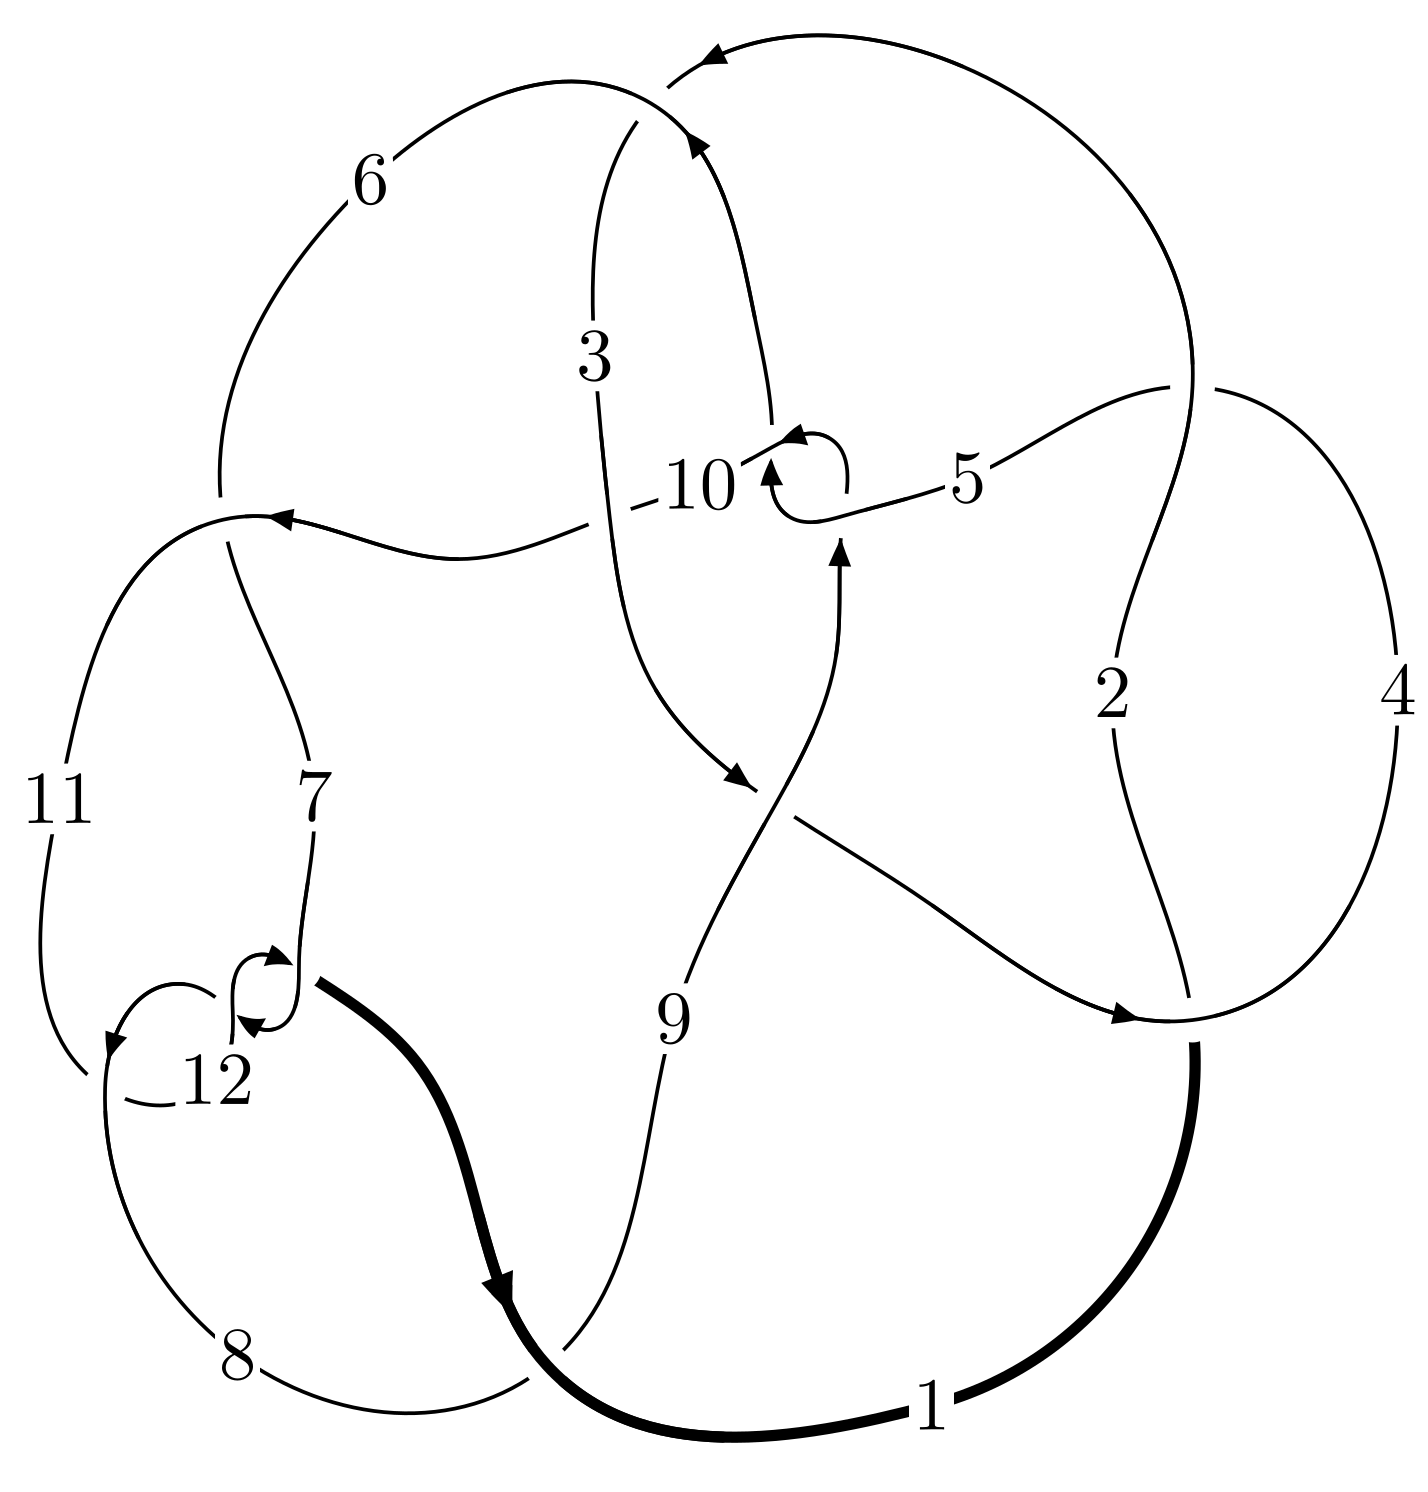
\includegraphics[width=112pt]{../../../GIT/diagram.site/Diagrams/png/1711_12a_0910.png}\\
\ \ \ A knot diagram\footnotemark}&
\allowdisplaybreaks
\textbf{Linearized knot diagam} \\
\cline{2-2}
 &
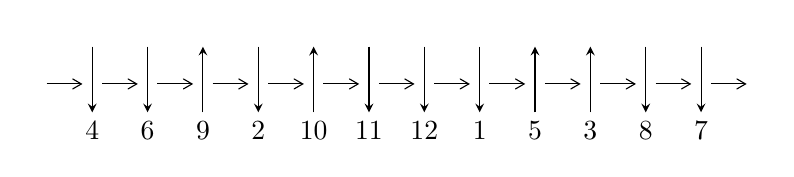
\begin{tikzpicture}[x=20pt, y=17pt]
	% nodes
	\node (C0) at (0, 0) {};
	\node (C1) at (1, 0) {};
	\node (C1U) at (1, +1) {};
	\node (C1D) at (1, -1) {4};

	\node (C2) at (2, 0) {};
	\node (C2U) at (2, +1) {};
	\node (C2D) at (2, -1) {6};

	\node (C3) at (3, 0) {};
	\node (C3U) at (3, +1) {};
	\node (C3D) at (3, -1) {9};

	\node (C4) at (4, 0) {};
	\node (C4U) at (4, +1) {};
	\node (C4D) at (4, -1) {2};

	\node (C5) at (5, 0) {};
	\node (C5U) at (5, +1) {};
	\node (C5D) at (5, -1) {10};

	\node (C6) at (6, 0) {};
	\node (C6U) at (6, +1) {};
	\node (C6D) at (6, -1) {11};

	\node (C7) at (7, 0) {};
	\node (C7U) at (7, +1) {};
	\node (C7D) at (7, -1) {12};

	\node (C8) at (8, 0) {};
	\node (C8U) at (8, +1) {};
	\node (C8D) at (8, -1) {1};

	\node (C9) at (9, 0) {};
	\node (C9U) at (9, +1) {};
	\node (C9D) at (9, -1) {5};

	\node (C10) at (10, 0) {};
	\node (C10U) at (10, +1) {};
	\node (C10D) at (10, -1) {3};

	\node (C11) at (11, 0) {};
	\node (C11U) at (11, +1) {};
	\node (C11D) at (11, -1) {8};

	\node (C12) at (12, 0) {};
	\node (C12U) at (12, +1) {};
	\node (C12D) at (12, -1) {7};
	\node (C13) at (13, 0) {};

	% arrows
	\draw[->,>={angle 60}]
	(C0) edge (C1) (C1) edge (C2) (C2) edge (C3) (C3) edge (C4) (C4) edge (C5) (C5) edge (C6) (C6) edge (C7) (C7) edge (C8) (C8) edge (C9) (C9) edge (C10) (C10) edge (C11) (C11) edge (C12) (C12) edge (C13) ;	\draw[->,>=stealth]
	(C1U) edge (C1D) (C2U) edge (C2D) (C3D) edge (C3U) (C4U) edge (C4D) (C5D) edge (C5U) (C6U) edge (C6D) (C7U) edge (C7D) (C8U) edge (C8D) (C9D) edge (C9U) (C10D) edge (C10U) (C11U) edge (C11D) (C12U) edge (C12D) ;
	\end{tikzpicture} \\
\hhline{~~} \\& 
\textbf{Solving Sequence} \\ \cline{2-2} 
 &
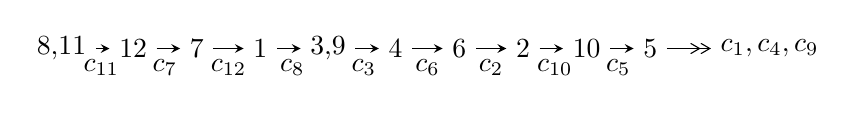
\begin{tikzpicture}[x=23pt, y=7pt]
	% node
	\node (A0) at (-1/8, 0) {8,11};
	\node (A1) at (1, 0) {12};
	\node (A2) at (2, 0) {7};
	\node (A3) at (3, 0) {1};
	\node (A4) at (65/16, 0) {3,9};
	\node (A5) at (41/8, 0) {4};
	\node (A6) at (49/8, 0) {6};
	\node (A7) at (57/8, 0) {2};
	\node (A8) at (65/8, 0) {10};
	\node (A9) at (73/8, 0) {5};
	\node (C1) at (1/2, -1) {$c_{11}$};
	\node (C2) at (3/2, -1) {$c_{7}$};
	\node (C3) at (5/2, -1) {$c_{12}$};
	\node (C4) at (7/2, -1) {$c_{8}$};
	\node (C5) at (37/8, -1) {$c_{3}$};
	\node (C6) at (45/8, -1) {$c_{6}$};
	\node (C7) at (53/8, -1) {$c_{2}$};
	\node (C8) at (61/8, -1) {$c_{10}$};
	\node (C9) at (69/8, -1) {$c_{5}$};
	\node (A10) at (11, 0) {$c_{1},c_{4},c_{9}$};

	% edge
	\draw[->,>=stealth]	
	(A0) edge (A1) (A1) edge (A2) (A2) edge (A3) (A3) edge (A4) (A4) edge (A5) (A5) edge (A6) (A6) edge (A7) (A7) edge (A8) (A8) edge (A9) ;
	\draw[->>,>={angle 60}]	
	(A9) edge (A10);
\end{tikzpicture} \\ 

\end{tabular} \\

\footnotetext{
The image of knot diagram is generated by the software ``\textbf{Draw programme}" developed by Andrew Bartholomew(\url{http://www.layer8.co.uk/maths/draw/index.htm\#Running-draw}), where we modified some parts for our purpose(\url{https://github.com/CATsTAILs/LinksPainter}).
}\phantom \\ \newline 
\centering \textbf{Ideals for irreducible components\footnotemark of $X_{\text{par}}$} 
 
\begin{align*}
I^u_{1}&=\langle 
-2.33082\times10^{48} u^{88}-4.60281\times10^{48} u^{87}+\cdots+1.09565\times10^{50} b+6.65254\times10^{48},\\
\phantom{I^u_{1}}&\phantom{= \langle  }2.18339\times10^{49} u^{88}+6.30025\times10^{49} u^{87}+\cdots+1.09565\times10^{50} a-1.77716\times10^{49},\;u^{89}+3 u^{88}+\cdots- u-1\rangle \\
\\
\end{align*}
\raggedright * 1 irreducible components of $\dim_{\mathbb{C}}=0$, with total 89 representations.\\
\footnotetext{All coefficients of polynomials are rational numbers. But the coefficients are sometimes approximated in decimal forms when there is not enough margin.}
\newpage
\renewcommand{\arraystretch}{1}
\centering \section*{I. $I^u_{1}= \langle -2.33\times10^{48} u^{88}-4.60\times10^{48} u^{87}+\cdots+1.10\times10^{50} b+6.65\times10^{48},\;2.18\times10^{49} u^{88}+6.30\times10^{49} u^{87}+\cdots+1.10\times10^{50} a-1.78\times10^{49},\;u^{89}+3 u^{88}+\cdots- u-1 \rangle$}
\flushleft \textbf{(i) Arc colorings}\\
\begin{tabular}{m{7pt} m{180pt} m{7pt} m{180pt} }
\flushright $a_{8}=$&$\begin{pmatrix}0\\u\end{pmatrix}$ \\
\flushright $a_{11}=$&$\begin{pmatrix}1\\0\end{pmatrix}$ \\
\flushright $a_{12}=$&$\begin{pmatrix}1\\u^2\end{pmatrix}$ \\
\flushright $a_{7}=$&$\begin{pmatrix}u\\u^3+u\end{pmatrix}$ \\
\flushright $a_{1}=$&$\begin{pmatrix}u^2+1\\u^4+2 u^2\end{pmatrix}$ \\
\flushright $a_{3}=$&$\begin{pmatrix}-0.199277 u^{88}-0.575022 u^{87}+\cdots-12.1043 u+0.162201\\0.0212733 u^{88}+0.0420097 u^{87}+\cdots+0.232993 u-0.0607175\end{pmatrix}$ \\
\flushright $a_{9}=$&$\begin{pmatrix}- u^5-2 u^3- u\\- u^7-3 u^5-2 u^3+u\end{pmatrix}$ \\
\flushright $a_{4}=$&$\begin{pmatrix}0.807980 u^{88}+1.04546 u^{87}+\cdots-11.7186 u-0.746785\\0.968268 u^{88}+2.19949 u^{87}+\cdots-0.339906 u-0.423067\end{pmatrix}$ \\
\flushright $a_{6}=$&$\begin{pmatrix}u^3+2 u\\u^3+u\end{pmatrix}$ \\
\flushright $a_{2}=$&$\begin{pmatrix}0.806563 u^{88}+1.17176 u^{87}+\cdots-12.2955 u+0.295786\\0.769539 u^{88}+1.76124 u^{87}+\cdots-0.106387 u-0.366511\end{pmatrix}$ \\
\flushright $a_{10}=$&$\begin{pmatrix}-0.0180093 u^{88}+0.190948 u^{87}+\cdots+1.30165 u-1.44754\\-0.0900530 u^{88}-0.276394 u^{87}+\cdots+0.505624 u+0.0372321\end{pmatrix}$ \\
\flushright $a_{5}=$&$\begin{pmatrix}-0.173831 u^{88}-0.158532 u^{87}+\cdots-1.02299 u+1.23980\\-0.433177 u^{88}-1.02726 u^{87}+\cdots+0.467787 u+0.155217\end{pmatrix}$\\&\end{tabular}
\flushleft \textbf{(ii) Obstruction class $= -1$}\\~\\
\flushleft \textbf{(iii) Cusp Shapes $= 2.69446 u^{88}+7.46992 u^{87}+\cdots-18.0671 u-6.35366$}\\~\\
\newpage\renewcommand{\arraystretch}{1}
\flushleft \textbf{(iv) u-Polynomials at the component}\newline \\
\begin{tabular}{m{50pt}|m{274pt}}
Crossings & \hspace{64pt}u-Polynomials at each crossing \\
\hline $$\begin{aligned}c_{1},c_{4}\end{aligned}$$&$\begin{aligned}
&u^{89}- u^{88}+\cdots- u+1
\end{aligned}$\\
\hline $$\begin{aligned}c_{2}\end{aligned}$$&$\begin{aligned}
&u^{89}-41 u^{88}+\cdots+975 u-239
\end{aligned}$\\
\hline $$\begin{aligned}c_{3}\end{aligned}$$&$\begin{aligned}
&u^{89}- u^{88}+\cdots+316117 u-39167
\end{aligned}$\\
\hline $$\begin{aligned}c_{5},c_{9}\end{aligned}$$&$\begin{aligned}
&u^{89}+u^{88}+\cdots+3 u+1
\end{aligned}$\\
\hline $$\begin{aligned}c_{6},c_{8}\end{aligned}$$&$\begin{aligned}
&u^{89}-3 u^{88}+\cdots+2879 u-1697
\end{aligned}$\\
\hline $$\begin{aligned}c_{7},c_{11},c_{12}\end{aligned}$$&$\begin{aligned}
&u^{89}+3 u^{88}+\cdots- u-1
\end{aligned}$\\
\hline $$\begin{aligned}c_{10}\end{aligned}$$&$\begin{aligned}
&u^{89}+3 u^{88}+\cdots- u-1
\end{aligned}$\\
\hline
\end{tabular}\\~\\
\newpage\renewcommand{\arraystretch}{1}
\flushleft \textbf{(v) Riley Polynomials at the component}\newline \\
\begin{tabular}{m{50pt}|m{274pt}}
Crossings & \hspace{64pt}Riley Polynomials at each crossing \\
\hline $$\begin{aligned}c_{1},c_{4}\end{aligned}$$&$\begin{aligned}
&y^{89}-61 y^{88}+\cdots-79 y-1
\end{aligned}$\\
\hline $$\begin{aligned}c_{2}\end{aligned}$$&$\begin{aligned}
&y^{89}-577 y^{88}+\cdots+4454365 y-57121
\end{aligned}$\\
\hline $$\begin{aligned}c_{3}\end{aligned}$$&$\begin{aligned}
&y^{89}-585 y^{88}+\cdots+115938293929 y-1534053889
\end{aligned}$\\
\hline $$\begin{aligned}c_{5},c_{9}\end{aligned}$$&$\begin{aligned}
&y^{89}-53 y^{88}+\cdots+9 y-1
\end{aligned}$\\
\hline $$\begin{aligned}c_{6},c_{8}\end{aligned}$$&$\begin{aligned}
&y^{89}-77 y^{88}+\cdots-33443983 y-2879809
\end{aligned}$\\
\hline $$\begin{aligned}c_{7},c_{11},c_{12}\end{aligned}$$&$\begin{aligned}
&y^{89}+71 y^{88}+\cdots+9 y-1
\end{aligned}$\\
\hline $$\begin{aligned}c_{10}\end{aligned}$$&$\begin{aligned}
&y^{89}+3 y^{88}+\cdots+65 y-1
\end{aligned}$\\
\hline
\end{tabular}\\~\\
\newpage\flushleft \textbf{(vi) Complex Volumes and Cusp Shapes}
$$\begin{array}{c|c|c}  
\text{Solutions to }I^u_{1}& \I (\text{vol} + \sqrt{-1}CS) & \text{Cusp shape}\\
 \hline 
\begin{aligned}
u &= -0.929512 + 0.135659 I \\
a &= \phantom{-}0.079974 - 0.661441 I \\
b &= -0.100252 - 0.483220 I\end{aligned}
 & -4.84729 + 0.69787 I & \phantom{-0.000000 } 0 \\ \hline\begin{aligned}
u &= -0.929512 - 0.135659 I \\
a &= \phantom{-}0.079974 + 0.661441 I \\
b &= -0.100252 + 0.483220 I\end{aligned}
 & -4.84729 - 0.69787 I & \phantom{-0.000000 } 0 \\ \hline\begin{aligned}
u &= \phantom{-}0.878375 + 0.106288 I \\
a &= -0.28997 + 1.92665 I \\
b &= -0.722394 + 1.077070 I\end{aligned}
 & -10.07520 - 6.99444 I & -11.18457 + 5.06210 I \\ \hline\begin{aligned}
u &= \phantom{-}0.878375 - 0.106288 I \\
a &= -0.28997 - 1.92665 I \\
b &= -0.722394 - 1.077070 I\end{aligned}
 & -10.07520 + 6.99444 I & -11.18457 - 5.06210 I \\ \hline\begin{aligned}
u &= -0.869045 + 0.102958 I \\
a &= -0.73422 - 2.38788 I \\
b &= -1.15331 - 1.15056 I\end{aligned}
 & -6.2758 + 13.0150 I & -7.65294 - 7.42348 I \\ \hline\begin{aligned}
u &= -0.869045 - 0.102958 I \\
a &= -0.73422 + 2.38788 I \\
b &= -1.15331 + 1.15056 I\end{aligned}
 & -6.2758 - 13.0150 I & -7.65294 + 7.42348 I \\ \hline\begin{aligned}
u &= \phantom{-}0.832380 + 0.027089 I \\
a &= -1.45814 - 2.69646 I \\
b &= -1.05310 - 1.65543 I\end{aligned}
 & -6.78345 - 3.76749 I & -10.75071 + 5.69816 I \\ \hline\begin{aligned}
u &= \phantom{-}0.832380 - 0.027089 I \\
a &= -1.45814 + 2.69646 I \\
b &= -1.05310 + 1.65543 I\end{aligned}
 & -6.78345 + 3.76749 I & -10.75071 - 5.69816 I \\ \hline\begin{aligned}
u &= -0.829253 + 0.008587 I \\
a &= -1.57002 + 0.97061 I \\
b &= -1.52106 + 0.53655 I\end{aligned}
 & -7.77581 + 0.24206 I & -12.35426 + 1.40830 I \\ \hline\begin{aligned}
u &= -0.829253 - 0.008587 I \\
a &= -1.57002 - 0.97061 I \\
b &= -1.52106 - 0.53655 I\end{aligned}
 & -7.77581 - 0.24206 I & -12.35426 - 1.40830 I\\
 \hline 
 \end{array}$$\newpage$$\begin{array}{c|c|c}  
\text{Solutions to }I^u_{1}& \I (\text{vol} + \sqrt{-1}CS) & \text{Cusp shape}\\
 \hline 
\begin{aligned}
u &= -0.825075 + 0.071584 I \\
a &= \phantom{-}1.21911 + 2.71232 I \\
b &= \phantom{-}1.31398 + 1.33937 I\end{aligned}
 & -1.75765 + 6.58893 I & -5.63761 - 6.42559 I \\ \hline\begin{aligned}
u &= -0.825075 - 0.071584 I \\
a &= \phantom{-}1.21911 - 2.71232 I \\
b &= \phantom{-}1.31398 - 1.33937 I\end{aligned}
 & -1.75765 - 6.58893 I & -5.63761 + 6.42559 I \\ \hline\begin{aligned}
u &= \phantom{-}0.038456 + 1.177140 I \\
a &= \phantom{-}1.58248 - 0.08343 I \\
b &= -1.184070 - 0.474407 I\end{aligned}
 & \phantom{-}0.95759 - 1.47026 I & \phantom{-0.000000 } 0 \\ \hline\begin{aligned}
u &= \phantom{-}0.038456 - 1.177140 I \\
a &= \phantom{-}1.58248 + 0.08343 I \\
b &= -1.184070 + 0.474407 I\end{aligned}
 & \phantom{-}0.95759 + 1.47026 I & \phantom{-0.000000 } 0 \\ \hline\begin{aligned}
u &= -0.648073 + 0.504252 I \\
a &= -0.241500 + 0.564840 I \\
b &= \phantom{-}0.232963 + 0.584124 I\end{aligned}
 & -3.63297 + 2.25684 I & -15.1399 - 9.7331 I \\ \hline\begin{aligned}
u &= -0.648073 - 0.504252 I \\
a &= -0.241500 - 0.564840 I \\
b &= \phantom{-}0.232963 - 0.584124 I\end{aligned}
 & -3.63297 - 2.25684 I & -15.1399 + 9.7331 I \\ \hline\begin{aligned}
u &= \phantom{-}0.810522 + 0.054674 I \\
a &= \phantom{-}0.13588 - 2.35750 I \\
b &= \phantom{-}0.489223 - 1.122630 I\end{aligned}
 & -4.87320 - 2.85130 I & -9.98435 + 3.35496 I \\ \hline\begin{aligned}
u &= \phantom{-}0.810522 - 0.054674 I \\
a &= \phantom{-}0.13588 + 2.35750 I \\
b &= \phantom{-}0.489223 + 1.122630 I\end{aligned}
 & -4.87320 + 2.85130 I & -9.98435 - 3.35496 I \\ \hline\begin{aligned}
u &= \phantom{-}0.790982\phantom{ +0.000000I} \\
a &= \phantom{-}15.7287\phantom{ +0.000000I} \\
b &= -0.113048\phantom{ +0.000000I}\end{aligned}
 & -3.96136\phantom{ +0.000000I} & \phantom{-}312.470\phantom{ +0.000000I} \\ \hline\begin{aligned}
u &= -0.485409 + 1.110780 I \\
a &= \phantom{-}0.090292 - 0.418240 I \\
b &= -0.202535 - 0.595275 I\end{aligned}
 & -1.86266 + 4.32433 I & \phantom{-0.000000 } 0\\
 \hline 
 \end{array}$$\newpage$$\begin{array}{c|c|c}  
\text{Solutions to }I^u_{1}& \I (\text{vol} + \sqrt{-1}CS) & \text{Cusp shape}\\
 \hline 
\begin{aligned}
u &= -0.485409 - 1.110780 I \\
a &= \phantom{-}0.090292 + 0.418240 I \\
b &= -0.202535 + 0.595275 I\end{aligned}
 & -1.86266 - 4.32433 I & \phantom{-0.000000 } 0 \\ \hline\begin{aligned}
u &= \phantom{-}0.064276 + 1.228880 I \\
a &= \phantom{-}0.842637 - 0.567641 I \\
b &= -0.552842 - 0.775586 I\end{aligned}
 & \phantom{-}1.44047 - 1.28035 I & \phantom{-0.000000 } 0 \\ \hline\begin{aligned}
u &= \phantom{-}0.064276 - 1.228880 I \\
a &= \phantom{-}0.842637 + 0.567641 I \\
b &= -0.552842 + 0.775586 I\end{aligned}
 & \phantom{-}1.44047 + 1.28035 I & \phantom{-0.000000 } 0 \\ \hline\begin{aligned}
u &= -0.762529 + 0.025248 I \\
a &= -0.356181 + 0.488600 I \\
b &= \phantom{-}0.280214 + 0.183737 I\end{aligned}
 & -2.21673 + 0.04211 I & -4.29235 + 0.75473 I \\ \hline\begin{aligned}
u &= -0.762529 - 0.025248 I \\
a &= -0.356181 - 0.488600 I \\
b &= \phantom{-}0.280214 - 0.183737 I\end{aligned}
 & -2.21673 - 0.04211 I & -4.29235 - 0.75473 I \\ \hline\begin{aligned}
u &= \phantom{-}0.509587 + 0.566712 I \\
a &= -0.821222 + 0.142653 I \\
b &= -0.758953 - 0.699859 I\end{aligned}
 & \phantom{-}0.25361 + 4.88837 I & -4.69859 - 4.12612 I \\ \hline\begin{aligned}
u &= \phantom{-}0.509587 - 0.566712 I \\
a &= -0.821222 - 0.142653 I \\
b &= -0.758953 + 0.699859 I\end{aligned}
 & \phantom{-}0.25361 - 4.88837 I & -4.69859 + 4.12612 I \\ \hline\begin{aligned}
u &= -0.431194 + 1.166650 I \\
a &= \phantom{-}0.847369 - 0.532968 I \\
b &= \phantom{-}1.07417 - 1.14245 I\end{aligned}
 & -3.01254 - 8.36103 I & \phantom{-0.000000 } 0 \\ \hline\begin{aligned}
u &= -0.431194 - 1.166650 I \\
a &= \phantom{-}0.847369 + 0.532968 I \\
b &= \phantom{-}1.07417 + 1.14245 I\end{aligned}
 & -3.01254 + 8.36103 I & \phantom{-0.000000 } 0 \\ \hline\begin{aligned}
u &= \phantom{-}0.444965 + 1.164420 I \\
a &= \phantom{-}0.625878 + 0.529751 I \\
b &= \phantom{-}0.604506 + 1.066130 I\end{aligned}
 & -6.82871 + 2.26796 I & \phantom{-0.000000 } 0\\
 \hline 
 \end{array}$$\newpage$$\begin{array}{c|c|c}  
\text{Solutions to }I^u_{1}& \I (\text{vol} + \sqrt{-1}CS) & \text{Cusp shape}\\
 \hline 
\begin{aligned}
u &= \phantom{-}0.444965 - 1.164420 I \\
a &= \phantom{-}0.625878 - 0.529751 I \\
b &= \phantom{-}0.604506 - 1.066130 I\end{aligned}
 & -6.82871 - 2.26796 I & \phantom{-0.000000 } 0 \\ \hline\begin{aligned}
u &= -0.366416 + 1.198290 I \\
a &= -1.304180 + 0.453304 I \\
b &= -1.15743 + 1.37009 I\end{aligned}
 & \phantom{-}1.69823 - 2.29157 I & \phantom{-0.000000 } 0 \\ \hline\begin{aligned}
u &= -0.366416 - 1.198290 I \\
a &= -1.304180 - 0.453304 I \\
b &= -1.15743 - 1.37009 I\end{aligned}
 & \phantom{-}1.69823 + 2.29157 I & \phantom{-0.000000 } 0 \\ \hline\begin{aligned}
u &= -0.113493 + 1.256270 I \\
a &= \phantom{-}0.060927 - 0.354565 I \\
b &= -0.207083 + 1.386810 I\end{aligned}
 & \phantom{-}3.23337 + 4.32643 I & \phantom{-0.000000 } 0 \\ \hline\begin{aligned}
u &= -0.113493 - 1.256270 I \\
a &= \phantom{-}0.060927 + 0.354565 I \\
b &= -0.207083 - 1.386810 I\end{aligned}
 & \phantom{-}3.23337 - 4.32643 I & \phantom{-0.000000 } 0 \\ \hline\begin{aligned}
u &= \phantom{-}0.352881 + 1.221590 I \\
a &= -0.714291 - 1.032090 I \\
b &= -0.330218 - 1.147620 I\end{aligned}
 & -1.28746 - 1.34293 I & \phantom{-0.000000 } 0 \\ \hline\begin{aligned}
u &= \phantom{-}0.352881 - 1.221590 I \\
a &= -0.714291 + 1.032090 I \\
b &= -0.330218 + 1.147620 I\end{aligned}
 & -1.28746 + 1.34293 I & \phantom{-0.000000 } 0 \\ \hline\begin{aligned}
u &= \phantom{-}0.569954 + 0.447706 I \\
a &= -0.133101 - 1.373890 I \\
b &= \phantom{-}0.935421 - 0.839804 I\end{aligned}
 & -0.10157 - 8.81133 I & -5.01759 + 9.13962 I \\ \hline\begin{aligned}
u &= \phantom{-}0.569954 - 0.447706 I \\
a &= -0.133101 + 1.373890 I \\
b &= \phantom{-}0.935421 + 0.839804 I\end{aligned}
 & -0.10157 + 8.81133 I & -5.01759 - 9.13962 I \\ \hline\begin{aligned}
u &= -0.038350 + 1.284690 I \\
a &= -2.58350 + 2.03136 I \\
b &= \phantom{-}0.066569 + 0.533918 I\end{aligned}
 & \phantom{-}4.40237 - 0.14969 I & \phantom{-0.000000 } 0\\
 \hline 
 \end{array}$$\newpage$$\begin{array}{c|c|c}  
\text{Solutions to }I^u_{1}& \I (\text{vol} + \sqrt{-1}CS) & \text{Cusp shape}\\
 \hline 
\begin{aligned}
u &= -0.038350 - 1.284690 I \\
a &= -2.58350 - 2.03136 I \\
b &= \phantom{-}0.066569 - 0.533918 I\end{aligned}
 & \phantom{-}4.40237 + 0.14969 I & \phantom{-0.000000 } 0 \\ \hline\begin{aligned}
u &= -0.330827 + 1.248950 I \\
a &= \phantom{-}0.624278 + 0.393456 I \\
b &= -0.113843 + 0.359168 I\end{aligned}
 & \phantom{-}1.57136 + 3.92056 I & \phantom{-0.000000 } 0 \\ \hline\begin{aligned}
u &= -0.330827 - 1.248950 I \\
a &= \phantom{-}0.624278 - 0.393456 I \\
b &= -0.113843 - 0.359168 I\end{aligned}
 & \phantom{-}1.57136 - 3.92056 I & \phantom{-0.000000 } 0 \\ \hline\begin{aligned}
u &= \phantom{-}0.376232 + 1.245480 I \\
a &= -0.86868 - 2.03778 I \\
b &= \phantom{-}1.15415 - 1.54424 I\end{aligned}
 & -3.01698 - 0.57611 I & \phantom{-0.000000 } 0 \\ \hline\begin{aligned}
u &= \phantom{-}0.376232 - 1.245480 I \\
a &= -0.86868 + 2.03778 I \\
b &= \phantom{-}1.15415 + 1.54424 I\end{aligned}
 & -3.01698 + 0.57611 I & \phantom{-0.000000 } 0 \\ \hline\begin{aligned}
u &= -0.374157 + 1.262040 I \\
a &= -0.25885 + 1.60552 I \\
b &= \phantom{-}1.58660 + 0.40293 I\end{aligned}
 & -3.88985 + 4.08284 I & \phantom{-0.000000 } 0 \\ \hline\begin{aligned}
u &= -0.374157 - 1.262040 I \\
a &= -0.25885 - 1.60552 I \\
b &= \phantom{-}1.58660 - 0.40293 I\end{aligned}
 & -3.88985 - 4.08284 I & \phantom{-0.000000 } 0 \\ \hline\begin{aligned}
u &= \phantom{-}0.345343 + 1.273650 I \\
a &= -6.63181 + 7.50024 I \\
b &= \phantom{-}0.128180 + 0.116605 I\end{aligned}
 & -0.00273 - 4.09240 I & \phantom{-0.000000 } 0 \\ \hline\begin{aligned}
u &= \phantom{-}0.345343 - 1.273650 I \\
a &= -6.63181 - 7.50024 I \\
b &= \phantom{-}0.128180 - 0.116605 I\end{aligned}
 & -0.00273 + 4.09240 I & \phantom{-0.000000 } 0 \\ \hline\begin{aligned}
u &= -0.373225 + 1.275880 I \\
a &= \phantom{-}0.538810 + 0.584956 I \\
b &= \phantom{-}1.45008 - 0.66232 I\end{aligned}
 & -3.78387 + 4.56362 I & \phantom{-0.000000 } 0\\
 \hline 
 \end{array}$$\newpage$$\begin{array}{c|c|c}  
\text{Solutions to }I^u_{1}& \I (\text{vol} + \sqrt{-1}CS) & \text{Cusp shape}\\
 \hline 
\begin{aligned}
u &= -0.373225 - 1.275880 I \\
a &= \phantom{-}0.538810 - 0.584956 I \\
b &= \phantom{-}1.45008 + 0.66232 I\end{aligned}
 & -3.78387 - 4.56362 I & \phantom{-0.000000 } 0 \\ \hline\begin{aligned}
u &= -0.067667 + 1.333310 I \\
a &= -0.999597 + 0.146870 I \\
b &= \phantom{-}0.676523 + 0.481566 I\end{aligned}
 & \phantom{-}4.84923 + 1.91577 I & \phantom{-0.000000 } 0 \\ \hline\begin{aligned}
u &= -0.067667 - 1.333310 I \\
a &= -0.999597 - 0.146870 I \\
b &= \phantom{-}0.676523 - 0.481566 I\end{aligned}
 & \phantom{-}4.84923 - 1.91577 I & \phantom{-0.000000 } 0 \\ \hline\begin{aligned}
u &= \phantom{-}0.158456 + 1.333150 I \\
a &= \phantom{-}0.151130 + 1.259860 I \\
b &= -1.053290 - 0.219247 I\end{aligned}
 & \phantom{-}8.12428 - 1.05571 I & \phantom{-0.000000 } 0 \\ \hline\begin{aligned}
u &= \phantom{-}0.158456 - 1.333150 I \\
a &= \phantom{-}0.151130 - 1.259860 I \\
b &= -1.053290 + 0.219247 I\end{aligned}
 & \phantom{-}8.12428 + 1.05571 I & \phantom{-0.000000 } 0 \\ \hline\begin{aligned}
u &= \phantom{-}0.375328 + 1.289580 I \\
a &= \phantom{-}1.65558 + 0.33666 I \\
b &= \phantom{-}0.95439 + 1.74592 I\end{aligned}
 & -2.68200 - 8.10808 I & \phantom{-0.000000 } 0 \\ \hline\begin{aligned}
u &= \phantom{-}0.375328 - 1.289580 I \\
a &= \phantom{-}1.65558 - 0.33666 I \\
b &= \phantom{-}0.95439 - 1.74592 I\end{aligned}
 & -2.68200 + 8.10808 I & \phantom{-0.000000 } 0 \\ \hline\begin{aligned}
u &= -0.321384 + 1.304160 I \\
a &= \phantom{-}0.577946 - 0.670078 I \\
b &= -0.482841 - 0.162336 I\end{aligned}
 & \phantom{-}1.94695 + 3.93362 I & \phantom{-0.000000 } 0 \\ \hline\begin{aligned}
u &= -0.321384 - 1.304160 I \\
a &= \phantom{-}0.577946 + 0.670078 I \\
b &= -0.482841 + 0.162336 I\end{aligned}
 & \phantom{-}1.94695 - 3.93362 I & \phantom{-0.000000 } 0 \\ \hline\begin{aligned}
u &= \phantom{-}0.106320 + 1.348410 I \\
a &= -1.41961 - 0.19552 I \\
b &= \phantom{-}1.34328 - 0.74955 I\end{aligned}
 & \phantom{-}8.74442 - 5.45639 I & \phantom{-0.000000 } 0\\
 \hline 
 \end{array}$$\newpage$$\begin{array}{c|c|c}  
\text{Solutions to }I^u_{1}& \I (\text{vol} + \sqrt{-1}CS) & \text{Cusp shape}\\
 \hline 
\begin{aligned}
u &= \phantom{-}0.106320 - 1.348410 I \\
a &= -1.41961 + 0.19552 I \\
b &= \phantom{-}1.34328 + 0.74955 I\end{aligned}
 & \phantom{-}8.74442 + 5.45639 I & \phantom{-0.000000 } 0 \\ \hline\begin{aligned}
u &= \phantom{-}0.359190 + 1.307950 I \\
a &= \phantom{-}1.12123 + 1.49982 I \\
b &= -0.613285 + 1.100380 I\end{aligned}
 & -0.61251 - 7.06495 I & \phantom{-0.000000 } 0 \\ \hline\begin{aligned}
u &= \phantom{-}0.359190 - 1.307950 I \\
a &= \phantom{-}1.12123 - 1.49982 I \\
b &= -0.613285 - 1.100380 I\end{aligned}
 & -0.61251 + 7.06495 I & \phantom{-0.000000 } 0 \\ \hline\begin{aligned}
u &= -0.367331 + 1.318480 I \\
a &= \phantom{-}0.99334 - 2.15790 I \\
b &= -1.42285 - 1.30244 I\end{aligned}
 & \phantom{-}2.59376 + 10.88130 I & \phantom{-0.000000 } 0 \\ \hline\begin{aligned}
u &= -0.367331 - 1.318480 I \\
a &= \phantom{-}0.99334 + 2.15790 I \\
b &= -1.42285 + 1.30244 I\end{aligned}
 & \phantom{-}2.59376 - 10.88130 I & \phantom{-0.000000 } 0 \\ \hline\begin{aligned}
u &= -0.388131 + 1.343150 I \\
a &= -1.03645 + 1.92373 I \\
b &= \phantom{-}1.21155 + 1.13898 I\end{aligned}
 & -1.7370 + 17.5280 I & \phantom{-0.000000 } 0 \\ \hline\begin{aligned}
u &= -0.388131 - 1.343150 I \\
a &= -1.03645 - 1.92373 I \\
b &= \phantom{-}1.21155 - 1.13898 I\end{aligned}
 & -1.7370 - 17.5280 I & \phantom{-0.000000 } 0 \\ \hline\begin{aligned}
u &= \phantom{-}0.393176 + 1.346290 I \\
a &= -0.96371 - 1.34947 I \\
b &= \phantom{-}0.808778 - 1.059800 I\end{aligned}
 & -5.51590 - 11.55620 I & \phantom{-0.000000 } 0 \\ \hline\begin{aligned}
u &= \phantom{-}0.393176 - 1.346290 I \\
a &= -0.96371 + 1.34947 I \\
b &= \phantom{-}0.808778 + 1.059800 I\end{aligned}
 & -5.51590 + 11.55620 I & \phantom{-0.000000 } 0 \\ \hline\begin{aligned}
u &= \phantom{-}0.157473 + 1.395500 I \\
a &= \phantom{-}1.280350 + 0.453034 I \\
b &= -1.120200 + 0.797498 I\end{aligned}
 & \phantom{-}5.76386 - 11.23110 I & \phantom{-0.000000 } 0\\
 \hline 
 \end{array}$$\newpage$$\begin{array}{c|c|c}  
\text{Solutions to }I^u_{1}& \I (\text{vol} + \sqrt{-1}CS) & \text{Cusp shape}\\
 \hline 
\begin{aligned}
u &= \phantom{-}0.157473 - 1.395500 I \\
a &= \phantom{-}1.280350 - 0.453034 I \\
b &= -1.120200 - 0.797498 I\end{aligned}
 & \phantom{-}5.76386 + 11.23110 I & \phantom{-0.000000 } 0 \\ \hline\begin{aligned}
u &= \phantom{-}0.08771 + 1.41474 I \\
a &= -0.454993 - 0.658545 I \\
b &= \phantom{-}0.839562 + 0.415887 I\end{aligned}
 & \phantom{-}6.64779 + 3.12890 I & \phantom{-0.000000 } 0 \\ \hline\begin{aligned}
u &= \phantom{-}0.08771 - 1.41474 I \\
a &= -0.454993 + 0.658545 I \\
b &= \phantom{-}0.839562 - 0.415887 I\end{aligned}
 & \phantom{-}6.64779 - 3.12890 I & \phantom{-0.000000 } 0 \\ \hline\begin{aligned}
u &= -0.42499 + 1.35409 I \\
a &= -0.247356 + 0.551362 I \\
b &= \phantom{-}0.355288 + 0.447703 I\end{aligned}
 & -0.19456 + 5.55020 I & \phantom{-0.000000 } 0 \\ \hline\begin{aligned}
u &= -0.42499 - 1.35409 I \\
a &= -0.247356 - 0.551362 I \\
b &= \phantom{-}0.355288 - 0.447703 I\end{aligned}
 & -0.19456 - 5.55020 I & \phantom{-0.000000 } 0 \\ \hline\begin{aligned}
u &= -0.18995 + 1.41013 I \\
a &= \phantom{-}0.602950 - 0.290908 I \\
b &= -0.635367 - 0.454422 I\end{aligned}
 & \phantom{-}2.47196 + 5.09965 I & \phantom{-0.000000 } 0 \\ \hline\begin{aligned}
u &= -0.18995 - 1.41013 I \\
a &= \phantom{-}0.602950 + 0.290908 I \\
b &= -0.635367 + 0.454422 I\end{aligned}
 & \phantom{-}2.47196 - 5.09965 I & \phantom{-0.000000 } 0 \\ \hline\begin{aligned}
u &= \phantom{-}0.376291 + 0.398020 I \\
a &= \phantom{-}0.095549 + 1.219570 I \\
b &= -1.033110 + 0.804997 I\end{aligned}
 & \phantom{-}3.36701 - 3.85907 I & -0.17251 + 7.32996 I \\ \hline\begin{aligned}
u &= \phantom{-}0.376291 - 0.398020 I \\
a &= \phantom{-}0.095549 - 1.219570 I \\
b &= -1.033110 - 0.804997 I\end{aligned}
 & \phantom{-}3.36701 + 3.85907 I & -0.17251 - 7.32996 I \\ \hline\begin{aligned}
u &= \phantom{-}0.431076 + 0.308197 I \\
a &= \phantom{-}1.59530 - 0.82053 I \\
b &= \phantom{-}0.826028 + 0.465822 I\end{aligned}
 & \phantom{-}3.09622 + 1.05401 I & -0.35608 + 2.55647 I\\
 \hline 
 \end{array}$$\newpage$$\begin{array}{c|c|c}  
\text{Solutions to }I^u_{1}& \I (\text{vol} + \sqrt{-1}CS) & \text{Cusp shape}\\
 \hline 
\begin{aligned}
u &= \phantom{-}0.431076 - 0.308197 I \\
a &= \phantom{-}1.59530 + 0.82053 I \\
b &= \phantom{-}0.826028 - 0.465822 I\end{aligned}
 & \phantom{-}3.09622 - 1.05401 I & -0.35608 - 2.55647 I \\ \hline\begin{aligned}
u &= -0.385829 + 0.181138 I \\
a &= \phantom{-}0.169374 - 1.094970 I \\
b &= \phantom{-}0.564988 - 1.049960 I\end{aligned}
 & -1.03006 + 2.56435 I & -8.07596 - 8.34971 I \\ \hline\begin{aligned}
u &= -0.385829 - 0.181138 I \\
a &= \phantom{-}0.169374 + 1.094970 I \\
b &= \phantom{-}0.564988 + 1.049960 I\end{aligned}
 & -1.03006 - 2.56435 I & -8.07596 + 8.34971 I \\ \hline\begin{aligned}
u &= -0.247836 + 0.309686 I \\
a &= \phantom{-}0.746852 - 0.804515 I \\
b &= -0.268178 - 0.518765 I\end{aligned}
 & -0.190615 + 0.890253 I & -4.19654 - 7.59118 I \\ \hline\begin{aligned}
u &= -0.247836 - 0.309686 I \\
a &= \phantom{-}0.746852 + 0.804515 I \\
b &= -0.268178 + 0.518765 I\end{aligned}
 & -0.190615 - 0.890253 I & -4.19654 + 7.59118 I \\ \hline\begin{aligned}
u &= \phantom{-}0.363950\phantom{ +0.000000I} \\
a &= -1.16034\phantom{ +0.000000I} \\
b &= \phantom{-}0.870754\phantom{ +0.000000I}\end{aligned}
 & -2.12362\phantom{ +0.000000I} & -9.50830\phantom{ +0.000000I} \\ \hline\begin{aligned}
u &= -0.133365 + 0.302895 I \\
a &= \phantom{-}4.60227 - 1.64086 I \\
b &= -0.405138 - 0.527039 I\end{aligned}
 & -0.202607 - 0.760168 I & \phantom{-}1.34645 - 9.24017 I \\ \hline\begin{aligned}
u &= -0.133365 - 0.302895 I \\
a &= \phantom{-}4.60227 + 1.64086 I \\
b &= -0.405138 + 0.527039 I\end{aligned}
 & -0.202607 + 0.760168 I & \phantom{-}1.34645 + 9.24017 I \\ \hline\begin{aligned}
u &= \phantom{-}0.315166\phantom{ +0.000000I} \\
a &= -1.87262\phantom{ +0.000000I} \\
b &= \phantom{-}0.632078\phantom{ +0.000000I}\end{aligned}
 & -2.14324\phantom{ +0.000000I} & -6.24080\phantom{ +0.000000I}\\
 \hline 
 \end{array}$$\newpage
\newpage\renewcommand{\arraystretch}{1}
\centering \section*{ II. u-Polynomials}
\begin{tabular}{m{50pt}|m{274pt}}
Crossings & \hspace{64pt}u-Polynomials at each crossing \\
\hline $$\begin{aligned}c_{1},c_{4}\end{aligned}$$&$\begin{aligned}
&u^{89}- u^{88}+\cdots- u+1
\end{aligned}$\\
\hline $$\begin{aligned}c_{2}\end{aligned}$$&$\begin{aligned}
&u^{89}-41 u^{88}+\cdots+975 u-239
\end{aligned}$\\
\hline $$\begin{aligned}c_{3}\end{aligned}$$&$\begin{aligned}
&u^{89}- u^{88}+\cdots+316117 u-39167
\end{aligned}$\\
\hline $$\begin{aligned}c_{5},c_{9}\end{aligned}$$&$\begin{aligned}
&u^{89}+u^{88}+\cdots+3 u+1
\end{aligned}$\\
\hline $$\begin{aligned}c_{6},c_{8}\end{aligned}$$&$\begin{aligned}
&u^{89}-3 u^{88}+\cdots+2879 u-1697
\end{aligned}$\\
\hline $$\begin{aligned}c_{7},c_{11},c_{12}\end{aligned}$$&$\begin{aligned}
&u^{89}+3 u^{88}+\cdots- u-1
\end{aligned}$\\
\hline $$\begin{aligned}c_{10}\end{aligned}$$&$\begin{aligned}
&u^{89}+3 u^{88}+\cdots- u-1
\end{aligned}$\\
\hline
\end{tabular}\newpage\renewcommand{\arraystretch}{1}
\centering \section*{ III. Riley Polynomials}
\begin{tabular}{m{50pt}|m{274pt}}
Crossings & \hspace{64pt}Riley Polynomials at each crossing \\
\hline $$\begin{aligned}c_{1},c_{4}\end{aligned}$$&$\begin{aligned}
&y^{89}-61 y^{88}+\cdots-79 y-1
\end{aligned}$\\
\hline $$\begin{aligned}c_{2}\end{aligned}$$&$\begin{aligned}
&y^{89}-577 y^{88}+\cdots+4454365 y-57121
\end{aligned}$\\
\hline $$\begin{aligned}c_{3}\end{aligned}$$&$\begin{aligned}
&y^{89}-585 y^{88}+\cdots+115938293929 y-1534053889
\end{aligned}$\\
\hline $$\begin{aligned}c_{5},c_{9}\end{aligned}$$&$\begin{aligned}
&y^{89}-53 y^{88}+\cdots+9 y-1
\end{aligned}$\\
\hline $$\begin{aligned}c_{6},c_{8}\end{aligned}$$&$\begin{aligned}
&y^{89}-77 y^{88}+\cdots-33443983 y-2879809
\end{aligned}$\\
\hline $$\begin{aligned}c_{7},c_{11},c_{12}\end{aligned}$$&$\begin{aligned}
&y^{89}+71 y^{88}+\cdots+9 y-1
\end{aligned}$\\
\hline $$\begin{aligned}c_{10}\end{aligned}$$&$\begin{aligned}
&y^{89}+3 y^{88}+\cdots+65 y-1
\end{aligned}$\\
\hline
\end{tabular}
\vskip 2pc
\end{document}